\documentclass{ximera}

\begin{document}
	\author{Stitz-Zeager}
	\xmtitle{TITLE}


\mfpicnumber{1}

\opengraphsfile{Polydivision}

\setcounter{footnote}{0}

\label{Polydivision}


In Section \ref{GraphsofPolynomials} we saw how much of the `local' behavior of the graph of a polynomial function is  determined by the zeros of the polynomial function.  In that section, the polynomial functions we were given were mostly, if not completely, factored which greatly simplified the process for determining zeros.  In this section, we revisit the relationship between zeros and factors with the ultimate aim of taking a polynomial function given to us in the form stated in Definition \ref{polynomialfunction}  and determining its zeros. 

\medskip

 We start by way of example:  suppose we wish to determine the zeros of  $f(x) = x^3 + 4x^2-5x-14$.  Setting $f(x)=0$ results in the polynomial equation $x^3 + 4x^2-5x-14=0$.   Despite all of the factoring techniques we learned (and forgot!) in Intermediate Algebra, this equation foils\footnote{pun intended} us at every turn. Knowing that the zeros of $f$ correspond to $x$-intercepts on the graph of $y=f(x)$, we use a graphing utility to produce the graph below on the left.  
 
 \medskip
 
 The graph suggests that the function has three zeros, one of which appears to be $x=2$ and two others for whom we are provided what we assume to be decimal approximations:  $x \approx -4.414$ and $x \approx -1.586$.    We can verify if these are zeros easily enough.   We find  $f(2) =(2)^2 + 4(2)^2-5(2)-14 = 0$,  but  $f(-4.414) \approx 0.0039$ and $f(-1.586) \approx 0.0022$,  While these last two values are probably by some measures,  `close' to $0$, they are not \textbf{exactly} equal to $0$.  The question becomes:  is there a way to use the fact that $x=2$ is a zero to obtain the other two zeros?  
 
 \medskip
 
 Based on our experience, if $x=2$ is a zero, it seems that there should be a factor of $(x-2)$ lurking around in the factorization of $f(x)$.  In other words, we should expect that $x^3 + 4x^2-5x-14=(x-2) \, q(x)$, where $q(x)$ is some other polynomial.  How could we find such a $q(x)$, if it even exists?  The answer comes from our old friend, polynomial division. (See Section \ref{polylongdiv}.) Below on the right, we perform the long division:  $(x^3 + 4x^2-5x-14) \div (x-2)$ and obtain $x^2+6x+7$.
 
 
 \medskip
 
 
\begin{tabular}{m{4in}m{2.5in}}

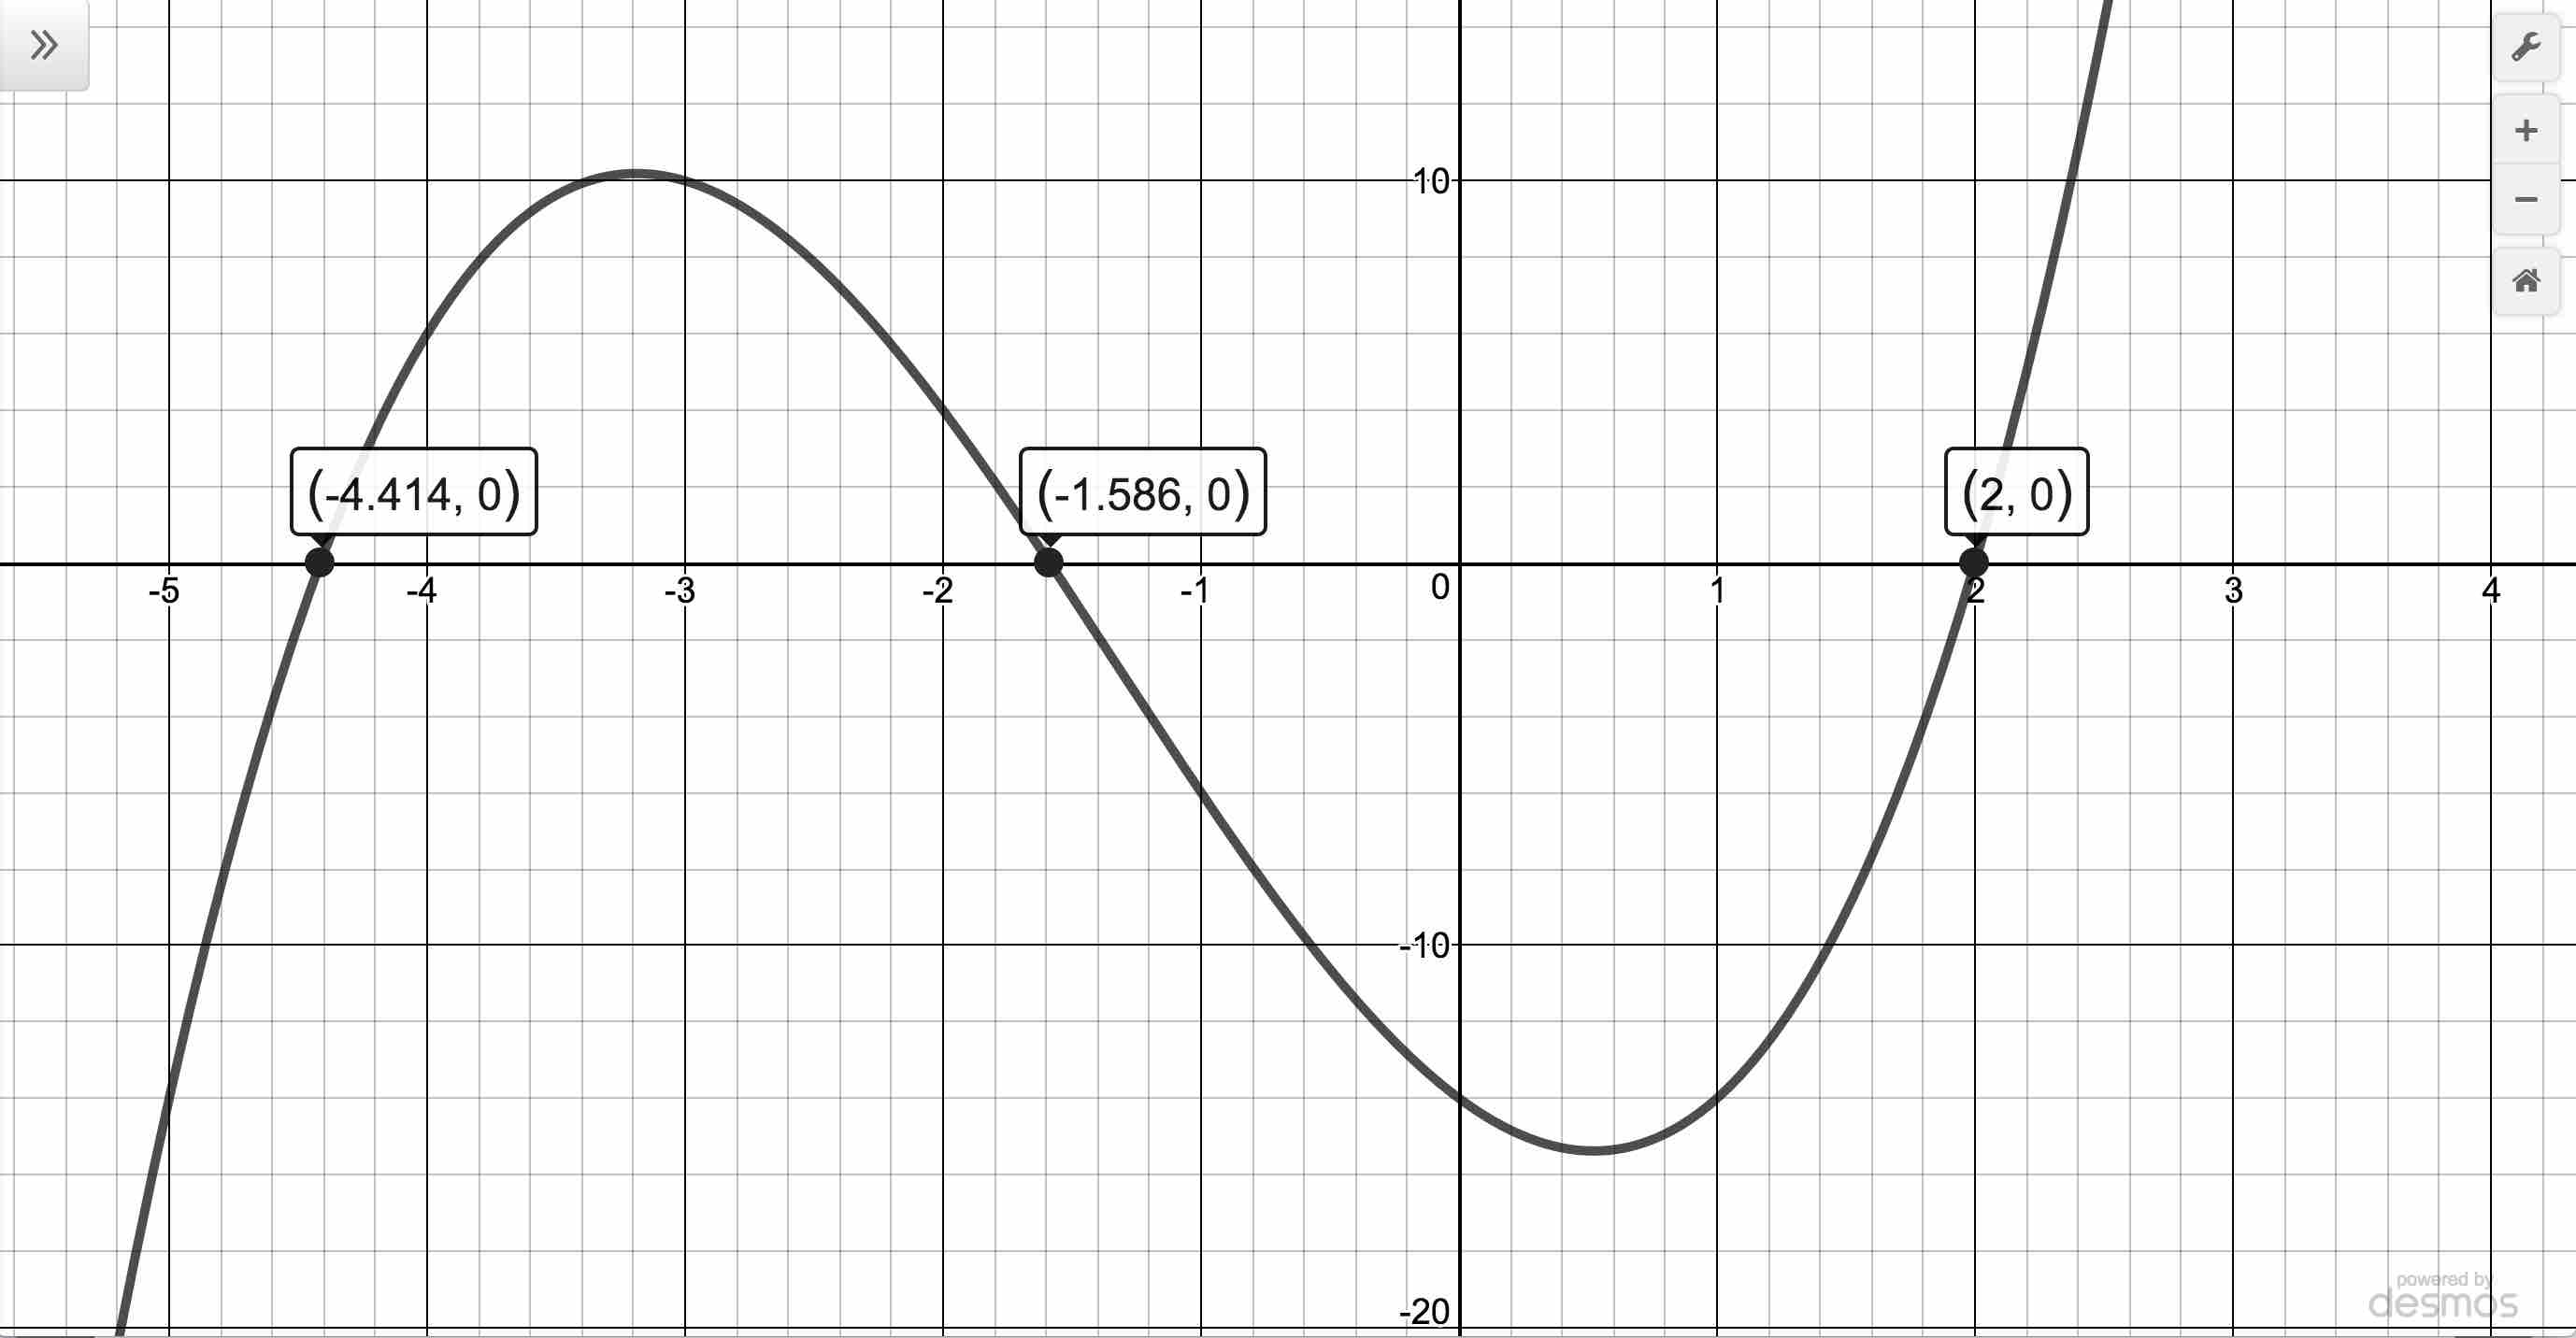
\includegraphics[height=2in]{./PolydivisionGraphics/PolyDiv01.jpg}

&

\setlength\arraycolsep{0.1pt}
\setlength\extrarowheight{2pt}

$\begin{array}{cccccccccc}

& & & & & x^2 & + & 6x & + & 7 \\ \hhline{~~~|-------}

x & - & 2 \, \vline& x^3 & + & 4x^2 & - & 5x & - & 14 \\

 &  &  -& \left(x^3 \right. & - & \left.  2x^2\right) &  &  &  &  \\ \hhline{~~~---~~~~} 
 &  &  &   &  & 6 x^2 & - & 5x &  &  \\ 
 &  &  &   & - & \left(6 x^2 \right. & - & \left. 12x \right) &  &  \\ \hhline{~~~~~---~~} 
 &  &  &   &   &  & & 7x  & - & 14 \\
 &  &  &   &   &  & - & \left( 7x \right. & - & \left. 14 \right) \\ \hhline{~~~~~~~---} 
 &   &  &  &  &  &  &  &  & 0
 
\end{array}$

\setlength\arraycolsep{5pt}
\setlength\extrarowheight{0pt}  \\

\end{tabular}



Said differently, $f(x) = x^3 + 4x^2-5x-14=(x-2)\left(x^2+6x+7\right)$.  Using this form of $f(x)$, we find the zeros by solving $(x-2)\left(x^2+6x+7\right)=0$.  Setting each factor equal to $0$, we get  $x-2=0$ (which gives us our known zero, $x=2$) as well as $x^2+6x+7=0$.   The latter doesn't factor nicely, so we apply the Quadratic Formula to get $x = -3 \pm \sqrt{2}$.  Sure enough, $-3 - \sqrt{2} \approx -4.414$ and $-3 +\sqrt{2} \approx -1.586$.  We leave it to the reader to show $f(-3-\sqrt{2}) = 0$ and $f(-3+\sqrt{2}) = 0$.  (See Exercise \ref{verifyrootsex}.) 

The point of this section is to generalize the technique applied here.  First up is a friendly reminder of what we can expect when we divide polynomials.

\smallskip

%% \colorbox{ResultColor}{\bbm

\begin{theorem} \label{polydivthm} \textbf{Polynomial Division:} 

Suppose $d(x)$ and $p(x)$ are nonzero polynomial functions where the degree of $p$ is greater than or equal to the degree of $d$.  There exist two unique polynomial functions, $q(x)$ and $r(x)$, such that $p(x) = d(x) \, q(x) + r(x),\,$ where either $r(x) = 0$ or the degree of $r$ is strictly less than the degree of $d$.
\end{theorem}
%% \ebm}

\medskip

As you may recall, all of the polynomials in Theorem \ref{polydivthm} have special names.  The polynomial $p$ is called the \index{polynomial division ! dividend} \textbf{dividend}; $d$ is the \index{polynomial division ! divisor} \textbf{divisor}; $q$ is the \index{polynomial division ! quotient} \textbf{quotient}; $r$ is the \index{polynomial division ! remainder} \textbf{remainder}.  If $r(x)=0$ then $d$ is called a \index{polynomial division ! factor} \textbf{factor} of $p$.  The word `unique' here is critical in that it guarantees there is only \textbf{one} quotient and remainder for each division problem.\footnote{Hence the use of the definite article `the' when speaking of \textbf{the} quotient and \textbf{the} remainder.} The proof of Theorem \ref{polydivthm} is usually relegated to a course in Abstract Algebra, but we can still use the result to establish two important facts which are the basis of the rest of the chapter.

\medskip

%% \colorbox{ResultColor}{\bbm

\begin{theorem} \label{remainderthm}\index{Remainder Theorem}\textbf{The Remainder Theorem:}  
Suppose $p$ is a polynomial function of degree at least $1$ and $c$ is a real number.  When $p(x)$ is divided by $x-c$ the remainder is $p(c)$.  Said differently, there is a polynomial  function $q(x)$ such that:  \[ p(x) = (x-c) q(x) + p(c)\]

\end{theorem}
%% \ebm}

\medskip


The proof of Theorem \ref{remainderthm} is a direct consequence of Theorem \ref{polydivthm}.  Since  $x-c$ has degree $1$, when a polynomial function is divided by $x-c$, the remainder is either $0$ or degree $0$ (i.e., a nonzero constant.)   In either case, $p(x) = (x-c) \, q(x) + r$, where $r$, the remainder, is a real number, possibly $0$.  It follows that $p(c) = (c-c) \, q(c) + r = 0 \cdot q(c) + r = r$, so we get $r = p(c)$ as required.  There is one last `low hanging fruit'\footnote{Jeff hates this expression and Carl included it just to annoy him.} to collect which we present below.

\medskip

%% \colorbox{ResultColor}{\bbm

\begin{theorem} \label{factorthm}\index{Factor Theorem}\textbf{The Factor Theorem:}  

Suppose $p$ is a nonzero polynomial function.  The real number $c$ is a zero of $p$ if and only if $(x-c)$ is a factor of $p(x)$.  

\end{theorem}
%% \ebm}

\medskip

Once again, we see the phrase `if and only if' which means there are really two things being said in  The Factor Theorem:  if $(x-c)$ is a factor of $p(x)$, then $c$ is a zero of $p$ and the \textbf{only} way $c$ is a zero  of $p$ is if $(x-c)$ is a factor of $p(x)$.  

\medskip

We argue the Factor Theorem as follows:   if $(x-c)$ is a factor of $p(x)$, then $p(x) = (x-c) \, q(x)$ for some polynomial $q$.  Hence, $p(c) = (c-c) \, q(c) = 0$, so $c$ is a zero of $p$.  Conversely, suppose $c$ is a zero of $p$, so $p(c) = 0$.   The Remainder Theorem tells us $p(x) = (x-c)q(x) + p(c) = (x-c)q(x) + 0 = (x-c)q(x)$.   Hence, $(x-c)$ is a factor of $p(x)$. 

\medskip

We have enough theory to explain why the concept of multiplicity (Definition \ref{multiplicity}) is well-defined. If $c$ is a zero of $p$, then The Factor Theorem tells us there is a polynomial function $q_{\text{\scriptsize $1$}}$ so that $p(x) = (x-c)q_{\text{\scriptsize $1$}}(x)$.  If $q_{\text{\scriptsize $1$}}(c) = 0$, then we apply the Factor Theorem to $q_{\text{\scriptsize $1$}}$ and find a  polynomial $q_{\text{\scriptsize $2$}}$ so that $q_{\text{\scriptsize $1$}}(x)  = (x-c) q_{\text{\scriptsize $2$}}(x)$.    Hence, we have  \[p(x) = (x-c) q_{\text{\scriptsize $1$}}(x) = (x-c) (x-c) q_{\text{\scriptsize $2$}}(x) = (x-c)^2 q_{\text{\scriptsize $2$}}(x).\]

\medskip

We now `rinse and repeat' this process.  Since the degree of $p$ is a finite number, this process has to end at some point.  That is we arrive at a factorization  $p(x) = (x-c)^m q(x)$ where $q(c) \neq 0$.  Suppose we arrive at a different factorization of $p$ using other methods.  That is, we find $p(x) = (x-c)^k Q(x)$, where $Q$ is a polynomial function with $Q(c) \neq 0$.   Then we have $(x-c)^m q(x) = (x-c)^k Q(x)$.    

\medskip

If $m \neq k$, then either $m<k$ or $m>k$.  If $m<k$, then we may divide both sides by $(x-c)^{m}$ to get: $q(x) = (x-c)^{k-m} Q(x)$.  Since $k>m$, $k-m>0$ and we would have $q(c) = (c-c)^{k-m} Q(c) = 0$, a contradiction since we are assuming $q(c) \neq 0$.   The assumption that $m>k$ likewise ends in a contradiction.   Therefore, we have $m = k$, so $p(x) = (x-c)^m q(x) = (x-c)^m Q(x)$.  By the uniqueness guaranteed in Theorem \ref{polydivthm}, we must have that $q(x) = Q(x)$.  Hence, the number $m$ and quotient polynomial $q(x)$ are unique. 

\medskip

The process outlined above, in which we coax out factors of $p(x)$ one at a time until we have all of them serves as a template for our work to come. Of the things The Factor Theorem tells us, the most pragmatic is that we had better find a more efficient way to divide polynomial functions by quantities of the form $x-c$.  Fortunately, people like \href{http://en.wikipedia.org/wiki/Synthetic_division}{\underline{Ruffini}} and \href{http://en.wikipedia.org/wiki/Horner_scheme}{\underline{Horner}} have already blazed this trail.  Let's take a closer look at the long division we performed at the beginning of the section and try to streamline it.  First off, let's change all of the subtractions into additions by distributing through the $-1$s.


\setlength\arraycolsep{0.1pt}
\setlength\extrarowheight{2pt}

\[ \begin{array}{cccccccccc}

& & & & & x^2 & + & 6x & + & 7 \\ \hhline{~~~|-------}

x & - & 2 \, \vline& x^3 & + & 4x^2 & - & 5x & - & 14 \\

 &  &  &  -x^3  & + &   2x^2 &  &  &  &  \\ \hhline{~~~---~~~~} 
 &  &  &   &  & 6 x^2 & - & 5x &  &  \\ 
 &  &  &   & &-6 x^2  & + &  12x &  &  \\ \hhline{~~~~~---~~} 
 &  &  &   &   &  & & 7x  & - & 14 \\
 &  &  &   &   &  & & - 7x  & + &  14  \\ \hhline{~~~~~~~---} 
 &   &  &  &  &  &  &  &  & 0
 
\end{array}\]

\setlength\arraycolsep{5pt}
\setlength\extrarowheight{0pt}


Next, observe that the terms $-x^3$, $-6x^2$ and $-7x$ are the exact opposite of the terms above them.  The algorithm we use ensures this is always the case, so we can omit them without losing any information.

\medskip

 Also note that the terms we `bring down' (namely the $-5x$ and $-14$) aren't really necessary to recopy, so we omit them, too.


\setlength\arraycolsep{0.1pt}
\setlength\extrarowheight{2pt}

\[ \begin{array}{cccccccccc}

& & & & & x^2 & + & 6x & + & 7 \\ \hhline{~~~|-------}

x & - & 2 \, \vline& \, \, x^3 & + & 4x^2 & - & 5x & - & 14 \\

 &  &  &   &  &   2x^2 &  &  &  &  \\ \hhline{~~~---~~~~} 
 &  &  &   &  & 6 x^2 &  &  &  &  \\ 
 &  &  &   & &  &  &  12x &  &  \\ \hhline{~~~~~---~~} 
 &  &  &   &   &  & & 7x  &  &  \\
 &  &  &   &   &  & &   &  &  14  \\ \hhline{~~~~~~~---} 
 &   &  &  &  &  &  &  &  & 0
 
\end{array}\]

\setlength\arraycolsep{5pt}
\setlength\extrarowheight{0pt}

Let's move terms up a bit and copy the $x^3$ into the last row.


\setlength\arraycolsep{0.1pt}
\setlength\extrarowheight{2pt}

\[ \begin{array}{cccccccccc}

& & & & & x^2 & + & 6x & + & 7 \\ \hhline{~~~|-------}

x & - & 2 \, \vline& \, \, x^3 & + & 4x^2 & - & 5x & - & 14 \\

 &  &  &   & &   2x^2 &  & 12x &  & 14 \\ \hhline{~~~-------} 
 &  &  & x^3  &  & 6 x^2 &  & 7x &  &0  \\  
\end{array}\]

\setlength\arraycolsep{5pt}
\setlength\extrarowheight{0pt}

Note that by arranging things in this manner, each term in the last row is obtained by adding the two terms above it.  Notice also that the quotient polynomial can be obtained by dividing each of the first three terms in the last row by $x$ and adding the results.   

\medskip

If you take the time to work back through the original division problem, you will find that this is exactly the way we determined the quotient polynomial.  This means that we no longer need to write the quotient polynomial down, nor the $x$ in the divisor, to determine our answer.

\setlength\arraycolsep{0.1pt}
\setlength\extrarowheight{2pt}

\[ \begin{array}{cccccccccc}


 & & - 2 \, \, \vline& \, \, x^3 & + & 4x^2 & - & 5x & - & 14 \\

 &  &  &   & &   2x^2 &  & 12x &  & 14 \\ \hhline{~~~-------} 
 &  &  & x^3  &  & 6 x^2 &  & 7x &  &0  \\  
\end{array}\]

\setlength\arraycolsep{5pt}
\setlength\extrarowheight{0pt}

We've streamlined things quite a bit so far, but we can still do more.  Let's take a moment to remind ourselves where the $2x^2$, $12x$ and $14$ came from in the second row.  Each of these terms was obtained by multiplying the terms in the quotient, $x^2$, $6x$ and $7$, respectively, by the $-2$ in $x-2$,  then by $-1$ when we changed the subtraction to addition. 

\medskip

 Multiplying by $-2$ then by $-1$ is the same as multiplying by $2$, so we replace the $-2$ in the divisor by $2$.   Furthermore, the coefficients of the quotient polynomial match the coefficients of the first three terms in the last row, so we now take the plunge and write only the coefficients of the terms to get



\[ \begin{array}{rrrrr}


  2 \, \, \vline& 1 & 4 & -5  & -14 \\

   &&   2 &   12 &   14 \\ \hhline{~----} 
  & 1  &   6  &  7 &  0  \\  
\end{array}\]



We have constructed a \index{polynomial division ! synthetic division}\index{synthetic division tableau}\textbf{synthetic division tableau} for this polynomial division problem.  Let's re-work our division problem using this tableau to see how it greatly streamlines the division process.  

\medskip

To divide $x^3+4x^2-5x-14$ by $x-2$, we write $2$ in the place of the divisor and the coefficients of $x^3+4x^2-5x-14$ in for the dividend.  Then `bring down' the first coefficient of the dividend.

\bigskip

\begin{center}

\begin{tabular}{cc}

$ \begin{array}{rrrrr}


  2 \, \, \vline& 1 & 4 & -5  & -14 \\

   &  &    &    &  \\ \hhline{~----} 
  &   &     &   &    \\  
\end{array}$  \hspace{1in}
&


$ \begin{array}{rrrrr}


  2 \, \, \vline& 1 & 4 & -5  & -14 \\

   & \downarrow &    &    &  \\ \hhline{~----} 
  & 1  &     &   &    \\  
\end{array}$ \\

\end{tabular}

\end{center}

\bigskip

Next, take the $2$ from the divisor and multiply by the $1$ that was `brought down' to get $2$.  Write this underneath the $4$, then add to get $6$.

\bigskip

\begin{center}

\begin{tabular}{cc}

$ \begin{array}{rrrrr}


  2 \, \, \vline& 1 & 4 & -5  & -14 \\

   & \downarrow  &  2  &    &  \\ \hhline{~----} 
  & 1  &     &   &    \\  
\end{array}$ \hspace{1in}
&


$ \begin{array}{rrrrr}


  2 \, \, \vline& 1 & 4 & -5  & -14 \\

   & \downarrow &  2  &    &  \\ \hhline{~----} 
  & 1  &   6  &   &    \\  
\end{array}$ \\


\end{tabular}

\end{center}

\bigskip

Now take the $2$ from the divisor times the $6$ to get $12$, and add it to the $-5$ to get $7$.

\bigskip

\begin{center}

\begin{tabular}{cc}


$ \begin{array}{rrrrr}


  2 \, \, \vline& 1 & 4 & -5  & -14 \\

   & \downarrow &  2  &  12  &  \\ \hhline{~----} 
  & 1  &   6  &   &    \\  
\end{array}$ \hspace{1in}

&

$ \begin{array}{rrrrr}


  2 \, \, \vline& 1 & 4 & -5  & -14 \\

   & \downarrow &  2  &  12  &  \\ \hhline{~----} 
  & 1  &   6  & 7  &    \\  
\end{array}$ \\


\end{tabular}

\end{center}


Finally, take the $2$ in the divisor times the $7$ to get $14$, and add it to the $-14$ to get $0$.

\bigskip

\begin{center}

\begin{tabular}{cc}

$ \begin{array}{rrrrr}


  2 \, \, \vline& 1 & 4 & -5  & -14 \\

   & \downarrow &  2  &  12  & 14 \\ \hhline{~----} 
  & 1  &   6  & 7  &    \\  
\end{array}$ \hspace{1in} 

&

$ \begin{array}{rrrrr}


  2 \, \, \vline& 1 & 4 & -5  & -14 \\

   & \downarrow &  2  &  12  & 14 \\ \hhline{~----} 
  & 1  &   6  & 7  &  \fbox{$0$}  \\  
\end{array}$ \\



\end{tabular}

\end{center}

The first three numbers in the last row of our tableau are the coefficients of the quotient polynomial.  Remember, we started with a third degree polynomial and divided by a first degree polynomial, so the quotient is a second degree polynomial.  Hence the quotient is $x^2+6x+7$.  

\medskip

The number in the box is the remainder.  Synthetic division is our tool of choice for dividing polynomials by divisors of the form $x-c$.  It is important to note that it works \textbf{only} for these kinds of divisors.\footnote{You'll need to use good old-fashioned polynomial long division for divisors of degree larger than 1.} 

\medskip

Also take note that when a polynomial (of degree at least $1$) is divided by $x-c$, the result will be a polynomial of exactly one less degree. Finally, it is  worth the time to trace each step in synthetic division back to its corresponding step in long division.  While the authors have done their best to indicate where the algorithm comes from, there is no substitute for working through it yourself.

\medskip

\begin{example}  Use synthetic division to perform the following polynomial divisions.  Identify the quotient and remainder. Write the dividend, quotient and remainder in the form given in Theorem \ref{polydivthm}.

\begin{multicols}{3}
\begin{enumerate}

\item  $\left(5x^3 - 2x^2 + 1\right) \div (x-3)$ \vphantom{$\dfrac{4-8x-12x^2}{2x-3}$}
\item  $\left(t^3+8\right) \div (t+2)$ \vphantom{$\dfrac{4-8x-12x^2}{2x-3}$}
\item  $\dfrac{4-8z-12z^2}{2z-3}$

\end{enumerate}
\end{multicols}

{ \bf Solution.} 

\begin{enumerate}


\item When setting up the synthetic division tableau, the coefficients of even `missing' terms need to be accounted for, so we enter $0$ for the coefficient of $x$ in the dividend.  

\[ \begin{array}{rrrrr}


  3 \, \, \vline& 5 & -2 & 0  & 1 \\

   & \downarrow &  15  &  39  & 117 \\ \hhline{~----} 
  & 5  &   13  & 39  &  \fbox{$118$}  \\  
\end{array}\]

Since the dividend was a third degree polynomial function, the quotient is a second degree (quadratic) polynomial function with coefficients $5$, $13$ and $39$:   $q(x) = 5x^2+13x+39$. The remainder is $r(x) = 118$.  According to Theorem \ref{polydivthm}, we have $5x^3 - 2x^2 + 1 = (x-3)\left(5x^2+13x+39 \right) + 118$, which we leave to the reader to check.

\item  To use synthetic division here, we rewrite $t+2$ as $t-(-2)$ and proceed as before

\[ \begin{array}{rrrrr}


  -2 \, \, \vline& 1 & 0 & 0  & 8 \\

   & \downarrow &  -2  &  4  & -8 \\ \hhline{~----} 
  & 1  &   -2  & 4  &  \fbox{$0$}  \\  
\end{array}\]

We get the quotient $q(t) = t^2-2t+4$ and the remainder $r(t) =0$. Relating the dividend, quotient and remainder gives: $t^3+8 = (t+2)\left( t^2-2t+4 \right)$, which is a specific instance of the `sum of cubes' formula some of you may recall from Intermediate Algebra.  

\item To divide $4-8z-12z^2$ by $2z-3$, two things must be done.  First, we write the dividend in descending powers of $z$ as $-12z^2-8z+4$.  Second, since synthetic division works only for factors of the form $z-c$, we factor $2z-3$ as $2\left(z-\frac{3}{2}\right)$.  Hence, we are dividing  $-12z^2-8z+4$ by two factors:  $2$ and $\left(z-\frac{3}{2}\right)$.  Dividing first by $2$, we obtain $-6z^2-4z+2$.  Next, we divide  $-6z^2-4z+2$ by $\left(z-\frac{3}{2}\right)$:

\[ \begin{array}{rrrr}


  \frac{3}{2} \, \, \vline& -6 & -4 & 2   \\ [4pt]

   & \downarrow &  -9  & -\frac{39}{2}  \\ [4pt] \hhline{~---} 
  &  -6  &   -13  & \fbox{$-\frac{35}{2}$}  \\  
\end{array}\]


Hence,  $-6z^2-4z+2 = \left(z-\frac{3}{2}\right)(-6 z - 13) - \frac{35}{2}$.  However when it comes to writing  the dividend, quotient and remainder in the form given in Theorem \ref{polydivthm}, we need to find $q(z)$ and $r(z)$ so that  $-12z^2-8z+4 = (2z-3) q(z) + r(z)$. Hence, starting with $-6z^2-4z+2 = \left(z-\frac{3}{2}\right)(-6 z - 13) - \frac{35}{2}$, we multiply $2$ back on both sides:  

\[ \begin{array}{rcl}
 -6z^2-4z+2  & = & \left(z-\frac{3}{2}\right)(-6 z - 13) - \frac{35}{2}\\
 2\left(-6z^2-4z+2 \right) & = & 2 \left[ \left(z-\frac{3}{2}\right)(-6 z - 13) - \frac{35}{2} \right] \\
 -12z^2-8z+4 & = & 2 \left(z-\frac{3}{2}\right)(-6 z - 13) - 2 \left(\frac{35}{2} \right) \\
 -12z^2-8z+4 & = & (2z-3) (-6 z - 13) - 35  \\ \end{array} \]

 At this stage, we have written $-12z^2-8z+4$ in the \textbf{form} $(2z-3) q(z) + r(z)$, so we identify the quotient as  $q(z) = -6z-13$ and the remainder is $r(z) = -35$.  
 
 \medskip
 
 But how can we be sure these are the same quotient and remainder polynomial functions we would have obtained if we had taken the time to do the long division in the first place?   Because of the word   `unique' in Theorem \ref{polydivthm}.  The theorem states that there is only \textbf{one} way to decompose $-12z^2-8z+4$ as $(2z-3)q(z) + r(z)$.  Since we have found such a way, we can be sure it is the only way.\footnote{But it wouldn't hurt to check, just this once.} \qed
\end{enumerate}

\end{example}

The next example pulls together all of the concepts discussed in this section.  

\begin{example} Let $p(x) = 2x^3-5x+3$.

\begin{enumerate}

\item  Find $p(-2)$ using The Remainder Theorem.  Check your answer by substitution.

\item  Verify  $x=1$ is a zero of $p$ and use this information to all the real zeros of $p$.

\end{enumerate}

{\bf Solution.}

\begin{enumerate}

\item  The Remainder Theorem states $p(-2)$ is the remainder when $p(x)$ is divided by $x-(-2)$.  We set up our synthetic division tableau below.  We are careful to record the coefficient of $x^2$ as $0$:

\[\begin{array}{rrrrr}
 -2 \, \, \vline& 2 & 0 & -5  & 3 \\

   & \downarrow &  -4  &  8  & -6 \\ \hhline{~----} 
  & 2  &   -4  & 3 &  \fbox{$-3$}  \\  
\end{array}\]

According to the Remainder Theorem, $p(-2) = -3$.  We can check this by direct substitution into the formula for $p(x)$:  $p(-2) = 2(-2)^3-5(-2)+3 = -16+10+3=-3$.

\item We verify $x=1$ is a zero of $p$ by evaluating $p(1) = 2(1)^3-5(1)+3 = 0$.  To see if there are any more real zeros, we need to solve $p(x) = 2x^3-5x+3 = 0$.  From the Factor Theorem, we know since $p(1) = 0$,  we can factor $p(x)$ as $(x-1)q(x)$.  To find $q(x)$, we use synthetic division:

\[\begin{array}{rrrrr}
 1 \, \, \vline& 2 & 0 & -5  & 3 \\

   & \downarrow &  2  &  2  & -3 \\ \hhline{~----} 
  & 2  &   2  & -3 &  \fbox{$0$}  \\  
\end{array}\]

As promised, our remainder is $0$, and we get  $p(x) = (x-1)\left( 2x^2 + 2x - 3\right)$.  Setting this form of $p(x)$ equal to  $0$ we get $(x-1)\left( 2x^2 + 2x - 3\right) = 0$.  We recover  $x = 1$ from setting $x-1=0$  but we also obtain $x = \frac{-1 \pm \sqrt{7}}{2}$ from  $2x^2 + 2x - 3=0$, courtesy of the Quadratic Formula.   \qed
\end{enumerate}
\end{example}

Our next example demonstrates how we can extend the synthetic division tableau to accommodate zeros of multiplicity greater than $1$.

\begin{example}  Let $p(x) = 4x^4-4x^3-11x^2+12x-3$. Show $x=\frac{1}{2}$ is a zero of multiplicity $2$ and find all of the remaining real zeros of $p$.


{\bf Solution.}  While computing $p\left(\frac{1}{2} \right) = 0$ shows $x=\frac{1}{2}$  is a zero of $p$, to prove it has multiplicity $2$, we need to factor $p(x) = \left(x - \frac{1}{2}\right)^2 q(x)$ with $q\left( \frac{1}{2} \right) \neq 0$,.   We set up for synthetic division, but instead of stopping after the first division, we continue the tableau downwards and divide $\left(x - \frac{1}{2}\right)$ directly into the quotient we obtained from the first division as follows:

\[\begin{array}{rrrrrr}
 \frac{1}{2} \, \, \vline& 4 & -4 & -11  & 12 & -3 \\

   & \downarrow &  2  &  -1  & -6 & 3\\ \hhline{~-----} 
   
  \frac{1}{2} \, \, \vline&  4  &   -2  & -12 & 6 &  \fbox{$0$}  \\
    
      & \downarrow &  2  &  0  & -6 &\\ \hhline{~----} 
      
       & 4  &   0  & -12 & \fbox{0} &   \\  



\end{array}\]

We get:\footnote{For those wanting more detail:  the first division gives:  $4x^4-4x^3-11x^2+12x-3=\left(x-\frac{1}{2}\right) \left(4x^3-2x^2-12x+6\right)$.  The second division gives: $4x^3-2x^2-12x+6=\left(x-\frac{1}{2}\right)\left(4x^2-12\right)$.}   $4x^4-4x^3-11x^2+12x-3 = \left(x-\frac{1}{2}\right)^2\left(4x^2-12\right)$.  Note if we let $q(x) = 4x^2-12$, then $q\left(\frac{1}{2} \right) = 4\left(\frac{1}{2} \right)^2 - 12 = -11 \neq 0$  which proves $x = \frac{1}{2}$ is a zero of $p$ of multiplicity $2$.   To find the remaining zeros of $p$, we set the quotient $4x^2-12=0$, so $x^2 = 3$ and extract square roots to get $x = \pm \sqrt{3}$.  \qed

\end{example}

A couple of things about the last example are worth mentioning. First, the extension of the synthetic division tableau for repeated divisions will be a common site in the sections to come. Typically, we will start with a higher order polynomial and peel off one zero at a time until we are left with a quadratic, whose roots can always be found using the Quadratic Formula.  

\medskip

Secondly, we found $x = \pm \sqrt{3}$ are zeros of $p$.  The Factor Theorem guarantees $\left(x-\sqrt{3}\right)$ and $\left(x - \left(-\sqrt{3}\right)\right)$ are both factors of $p$.  We can certainly put the Factor Theorem to the test and continue the synthetic division tableau from above to see what happens.

\[\begin{array}{rrrrrr}
 \frac{1}{2} \, \, \vline& 4 & -4 & -11  & 12 & -3 \\

  & \downarrow &  2  &  -1  & -6 & 3\\ \hhline{~-----} 
  
  \frac{1}{2} \, \, \vline&  4  &   -2  & -12 & 6 &  \fbox{$0$}  \\
    
  & \downarrow &  2  &  0  & -6 &\\ \hhline{~----} 
 
  
 \sqrt{3} \, \, \vline  & 4  &   0  & -12 & \fbox{0} &   \\
  
                        & \downarrow &  4\sqrt{3}  & 12  & &\\ \hhline{~---} 
 
   -\sqrt{3} \, \, \vline  & 4  &  4\sqrt{3}  & \fbox{0} &  &   \\  
       
                          & \downarrow &  -4\sqrt{3}  &   & &\\ \hhline{~--} 
       
													& 4  &  \fbox{0}  &  &  &   \\

\end{array}\]

This gives us

 \[\begin{array}{rcl} 
 
 p(x) & = &  4x^4-4x^3-11x^2+12x-3 \\
        & = & \left(x-\frac{1}{2}\right)^2 \left(x-\sqrt{3}\right)\left(x - \left(-\sqrt{3}\right)\right) (4) \\
        & = &  4\left(x-\frac{1}{2}\right)^2 \left(x-\sqrt{3}\right)\left(x - \left(-\sqrt{3}\right)\right) \\ \end{array} \]

We have shown that $p$ is a product of its leading coefficient times linear factors of the form $(x-c)$ where $c$ are zeros of $p$. It may surprise and delight the reader that, in theory, all polynomials can be reduced to this kind of factorization.  We leave that discussion to Section \ref{ComplexZeros}, because the zeros may not be real numbers.  Our final theorem in the section gives us an upper bound on the number of real zeros. 

\medskip

%% \colorbox{ResultColor}{\bbm
\begin{theorem}  \label{nzerosreal} 

Suppose $f$ is a polynomial of degree $n \geq 1$.  Then $f$ has at most $n$ real zeros, counting multiplicities.

\end{theorem}
%% \ebm}

\medskip

Theorem \ref{nzerosreal} is a consequence of the Factor Theorem and polynomial multiplication.  Every zero $c$ of $f$ gives us a factor of the form $(x-c)$ for $f(x)$.  Since $f$ has degree $n$, there can be at most $n$ of these factors.  The next section provides us some tools which not only help us determine where the real zeros are to be found, but which real numbers they may be.

\medskip

We close this section with a summary of several concepts previously presented.  You should take the time to look back through the text to see where each concept was first introduced and where each connection to the other concepts was made.

\medskip

%% \colorbox{ResultColor}{\bbm

\centerline{\textbf{Connections Between Zeros, Factors and Graphs of Polynomial Functions}}

\medskip

\hspace{.17in} Suppose $p$ is a polynomial function of degree $n \geq 1$.  The following statements are equivalent:

\begin{itemize}

\item The real number $c$ is a zero of $p$
\item $p(c) = 0$
\item $x = c$ is a solution to the polynomial equation $p(x) = 0$
\item $(x - c)$ is a factor of $p(x)$
\item The point $(c, 0)$ is an $x$-intercept of the graph of $y = p(x)$

\end{itemize}

%% \ebm}

\newpage

\subsection{Exercises}

%% SKIPPED %% 
In Exercises \ref{synthdivreviewfirst} - \ref{synthdivreviewlast}, use synthetic division to perform the following polynomial divisions.  Identify the quotient and remainder. Write the divisor, quotient and remainder in the form given in Theorem \ref{polydivthm}.

\begin{multicols}{2}
\begin{enumerate}


\item $\left(3x^2-2x+1 \right) \div \left(x-1\right)$ \label{synthdivreviewfirst}
\item $\left(x^2-5 \right) \div \left(x-5\right)$

\setcounter{HW}{\value{enumi}}
\end{enumerate}
\end{multicols}

\begin{multicols}{2}
\begin{enumerate}
\setcounter{enumi}{\value{HW}}

\item $\left(3-4t-2t^2 \right) \div \left(t+1\right)$
\item $\left(4t^2-5t +3\right) \div \left(t+3\right)$

\setcounter{HW}{\value{enumi}}
\end{enumerate}
\end{multicols}

\begin{multicols}{2}
\begin{enumerate}
\setcounter{enumi}{\value{HW}}

\item $\left(z^3 + 8 \right) \div \left(z+2\right)$
\item $\left(4z^3 +2z-3 \right) \div \left(z -3\right)$

\setcounter{HW}{\value{enumi}}
\end{enumerate}
\end{multicols}

\begin{multicols}{2}
\begin{enumerate}
\setcounter{enumi}{\value{HW}}

\item $\left(18x^2-15x-25\right) \div \left(x - \frac{5}{3} \right)$
\item $\left(4x^2-1 \right) \div \left(x - \frac{1}{2} \right)$

\setcounter{HW}{\value{enumi}}
\end{enumerate}
\end{multicols}

\begin{multicols}{2}
\begin{enumerate}
\setcounter{enumi}{\value{HW}}

\item $\left(2t^3+t^2+2t+1 \right) \div \left(t + \frac{1}{2} \right)$
\item $\left(3t^3 - t + 4 \right) \div \left(t - \frac{2}{3} \right)$

\setcounter{HW}{\value{enumi}}
\end{enumerate}
\end{multicols}

\begin{multicols}{2}
\begin{enumerate}
\setcounter{enumi}{\value{HW}}

\item $\left(2z^3 - 3z +1 \right) \div \left(z - \frac{1}{2} \right)$
\item $\left(4z^4-12z^3+13z^2 -12z+9\right) \div \left(z - \frac{3}{2} \right)$

\setcounter{HW}{\value{enumi}}
\end{enumerate}
\end{multicols}

\begin{multicols}{2}
\begin{enumerate}
\setcounter{enumi}{\value{HW}}

\item $\left(x^4-6x^2+9 \right) \div \left(x -\sqrt{3} \right)$
\item $\left(x^6-6x^4+12x^2-8\right) \div \left(x +\sqrt{2} \right)$ \label{synthdivreviewlast}

\setcounter{HW}{\value{enumi}}
\end{enumerate}
\end{multicols}

In Exercises \ref{remainderexerfirst} - \ref{remainderexerlast}, find $p(c)$ using the Remainder Theorem.  If $p(c) = 0$, use the Factor Theorem to partially factor the polynomial function.

\begin{multicols}{2}
\begin{enumerate}
\setcounter{enumi}{\value{HW}}

\item $p(x) = 2x^2 - x + 1$, $c = 4$ \label{remainderexerfirst}
\item $p(x) = 4x^2-33x-180$, $c = 12$

\setcounter{HW}{\value{enumi}}
\end{enumerate}
\end{multicols}


\begin{multicols}{2}
\begin{enumerate}
\setcounter{enumi}{\value{HW}}

\item $p(t) = 2t^3 - t + 6$, $c=-3$
\item $p(t) = t^3+2t^2+3t+4$, $c =-1$

\setcounter{HW}{\value{enumi}}
\end{enumerate}
\end{multicols}

\begin{multicols}{2}
\begin{enumerate}
\setcounter{enumi}{\value{HW}}

\item $p(z) =3z^3-6z^2+4z-8$, $c=2$
\item $p(z) = 8z^3+12z^2+6z+1$, $c =-\frac{1}{2}$

\setcounter{HW}{\value{enumi}}
\end{enumerate}
\end{multicols}

\begin{multicols}{2}
\begin{enumerate}
\setcounter{enumi}{\value{HW}}

\item $p(x) = x^4 - 2x^2+4$, $c=\frac{3}{2}$
\item $p(x) = 6x^4-x^2+2$, $c =-\frac{2}{3}$

\setcounter{HW}{\value{enumi}}
\end{enumerate}
\end{multicols}


\begin{multicols}{2}
\begin{enumerate}
\setcounter{enumi}{\value{HW}}

\item $p(t) = t^4 +t^3-6t^2-7t-7$, $c=-\sqrt{7}$
\item $p(t) = t^2-4t+1$, $c =2-\sqrt{3}$ \label{remainderexerlast}

\setcounter{HW}{\value{enumi}}
\end{enumerate}
\end{multicols}



In Exercises \ref{factorpolyzerofirst} - \ref{factorpolyzerolast}, you are given a polynomial function and one of its zeros.  Find the remaining real zeros and factor the polynomial.  

\begin{multicols}{2}
\begin{enumerate}
\setcounter{enumi}{\value{HW}}

\item $x^{3} - 6x^{2} + 11x - 6, \;\; c = 1$ \label{factorpolyzerofirst}
\item $x^{3} - 24x^{2} + 192x - 512, \;\; c = 8$

\setcounter{HW}{\value{enumi}}
\end{enumerate}
\end{multicols}

\begin{multicols}{2}
\begin{enumerate}
\setcounter{enumi}{\value{HW}}

\item $3t^{3} + 4t^{2} - t - 2, \;\; c = \frac{2}{3}$
\item $2t^3-3t^2-11t+6, \;\; c=\frac{1}{2}$

\setcounter{HW}{\value{enumi}}
\end{enumerate}
\end{multicols}

\begin{multicols}{2}
\begin{enumerate}
\setcounter{enumi}{\value{HW}}

\item $z^3+2z^2-3z-6, \;\; c = -2$
\item $2z^3-z^2-10z+5, \;\; c=\frac{1}{2}$

\setcounter{HW}{\value{enumi}}
\end{enumerate}
\end{multicols}

\vspace*{-0.2in}
\enlargethispage{0.2in}
\begin{enumerate}
\setcounter{enumi}{\value{HW}}

\item $4x^{4} - 28x^{3} + 61x^{2} - 42x + 9$, $c = \frac{1}{2}$ is a zero of multiplicity 2 

\item  $t^5+2t^4-12t^3-38t^2-37t-12$, $c=-1$ is a zero of multiplicity 3

\item $125z^{5} - 275z^{4} - 2265z^{3} - 3213z^{2} - 1728z - 324$, $c = -\frac{3}{5}$ is a zero of multiplicity 3

\item $x^{2} - 2x - 2, \;\; c = 1 - \sqrt{3}$ \label{factorpolyzerolast}

\setcounter{HW}{\value{enumi}}
\end{enumerate}


\begin{enumerate}
\setcounter{enumi}{\value{HW}}

\item Find a quadratic polynomial with \underline{integer} coefficients which has $x = \dfrac{3}{5} \pm \dfrac{\sqrt{29}}{5}$ as its real zeros.

\item  \label{verifyrootsex}  For $f(x) = x^3 + 4x^2-5x-14$, show $f(-3-\sqrt{2}) = 0$ and $f(-3+\sqrt{2}) = 0$ two ways:

\begin{enumerate}

\item  By direct substitution.

\item  Using synthetic division and the Factor Theorem

\end{enumerate}

\item  \label{oneisazeroex} Let $f(x) = a_{n} x^{n} + a_{n-\mbox{\tiny$1$}} x^{n-\mbox{\tiny$1$}} + \ldots + a_{\mbox{\tiny $2$}} x^{\mbox{\tiny $2$}} + a_{\mbox{\tiny $1$}} x + a_{\mbox{\tiny $0$}}$ be a polynomial function with the property that $ a_{n}+a_{n-\mbox{\tiny$1$}} + \ldots + a_{\mbox{\tiny $1$}} + a_{\mbox{\tiny $0$}} = 0$.  (That is, the sum of the coefficients and the constant term is $0$.)  

Prove that $(x-1)$ is a factor of $f(x)$.

HINT:  Show $f(1) = 0$ and invoke the Factor Theorem

\item  Verify the result in number \ref{oneisazeroex} with the functions: $f(x) = x^3 - 2x + 1$ and  $f(x) = 3x^4-x-2$.

\item  \label{monomialdiffquotex} Suppose $a$ is a nonzero real number.  Find the quotients below, using synthetic division as required. 

\begin{multicols}{5}
\begin{itemize}

\item $\dfrac{x - a}{x-a}$ 

\item $\dfrac{x^2 - a^2}{x-a}$ 

\item $\dfrac{x^3 - a^3}{x-a}$ 

\item $\dfrac{x^4 - a^4}{x-a}$ 

\item $\dfrac{x^5 - a^5}{x-a}$ 


\end{itemize}

\end{multicols}

Based on the pattern that evolves, find the quotient: $\dfrac{x^{10} - a^{10}}{x-a}$.  What about  $\dfrac{x^{n} - a^{n}}{x-a}$?


\item  \label{geoseriespreview} Use your result from number \ref{monomialdiffquotex} to rewrite the sum: $1 + r + r^2 + \dots + r^{n-2} + r^{n-1}$ as a quotient. What assumptions need to be made about $r$?

\setcounter{HW}{\value{enumi}}
\end{enumerate}

\newpage

\subsection{Answers}


\begin{enumerate}

\item $\left(3x^2-2x+1 \right) = \left(x-1\right) (3x+1)+2$
\item $\left(x^2-5 \right)= \left(x-5\right)(x+5) + 20$


\item $\left(3-4t-2t^2 \right) = \left(t+1\right)(-2t-2)+5$
\item $\left(4t^2-5t +3\right) = \left(t+3\right)(4t-17)+54$


\item $\left(z^3 + 8 \right) = \left(z+2\right) \left(z^2-2z+4\right) + 0$
\item $\left(4z^3 +2z-3 \right) = \left(z -3\right) \left(4z^2+12z+38\right) + 111$


\item $\left(18x^2-15x-25\right) = \left(x - \frac{5}{3} \right)(18x+15)+0$
\item $\left(4x^2-1 \right) = \left(x - \frac{1}{2} \right)(4x+2)+0$


\item $\left(2t^3+t^2+2t+1 \right) = \left(t + \frac{1}{2} \right)\left(2t^2+2\right)+0$
\item $\left(3t^3 - t + 4 \right) = \left(t - \frac{2}{3} \right) \left(3t^2+2t+\frac{1}{3}\right) + \frac{38}{9}$


\item $\left(2z^3 - 3z +1 \right) = \left(z - \frac{1}{2} \right) \left(2z^2+z-\frac{5}{2}\right)-\frac{1}{4}$
\item $\left(4z^4-12z^3+13z^2 -12z+9\right) = \left(z - \frac{3}{2} \right) \left(4z^3-6z^2+4z-6 \right)+0$

\item $\left(x^4-6x^2+9 \right) = \left(x -\sqrt{3} \right) \left(x^3+\sqrt{3} \,x^2-3x-3\sqrt{3}\right) + 0$
\item $\left(x^6-6x^4+12x^2-8\right) = \left(x +\sqrt{2} \right) \left(x^5-\sqrt{2} \, x^4-4x^3+4\sqrt{2} \, x^2+4x-4\sqrt{2}\right) + 0$


\setcounter{HW}{\value{enumi}}
\end{enumerate}

\begin{multicols}{2}
\begin{enumerate}
\setcounter{enumi}{\value{HW}}

\item $p(4) = 29$
\item $p(12) =0$, $p(x) = (x-12)(4x+15)$

\setcounter{HW}{\value{enumi}}
\end{enumerate}
\end{multicols}


\begin{multicols}{2}
\begin{enumerate}
\setcounter{enumi}{\value{HW}}

\item $p(-3)=-45$
\item $p(-1)=2$

\setcounter{HW}{\value{enumi}}
\end{enumerate}
\end{multicols}

\begin{multicols}{2}
\begin{enumerate}
\setcounter{enumi}{\value{HW}}

\item $p(2) =0$, $p(z)= (z-2) \left(3z^2+4\right)$
\item $p\left(-\frac{1}{2}\right) = 0$, $p(z)  = \left(z+\frac{1}{2}\right)\left(8z^2+8z+2\right)$

\setcounter{HW}{\value{enumi}}
\end{enumerate}
\end{multicols}

\begin{multicols}{2}
\begin{enumerate}
\setcounter{enumi}{\value{HW}}

\item $p\left(\frac{3}{2}\right) = \frac{73}{16}$
\item $p\left(-\frac{2}{3}\right) = \frac{74}{27}$

\setcounter{HW}{\value{enumi}}
\end{enumerate}
\end{multicols}

\begin{enumerate}
\setcounter{enumi}{\value{HW}}

\item $p(-\sqrt{7}) = 0$, $p(t) = (t+\sqrt{7})\left(t^3+(1-\sqrt{7}) t^2+(1-\sqrt{7})t-\sqrt{7}  \right)$
\item $p(2-\sqrt{3}) =0$, $p(t) = (t-(2-\sqrt{3}))(t-(2+\sqrt{3})) $

\setcounter{HW}{\value{enumi}}
\end{enumerate}

\begin{enumerate}
\setcounter{enumi}{\value{HW}}

\item $x^{3} - 6x^{2} + 11x - 6 = (x - 1)(x - 2)(x - 3)$
\item $x^{3} - 24x^{2} + 192x - 512 = (x - 8)^{3}$
\item $3t^{3} + 4t^{2} - t - 2 = 3\left(t - \frac{2}{3}\right)(t + 1)^{2}$

\item $2t^3-3t^2-11t+6 = 2\left(t-\frac{1}{2}\right)(t+2)(t-3)$

\item $z^3+2z^2-3z-6 = (z+2)(z+\sqrt{3})(z-\sqrt{3})$
\item $2z^3-z^2-10z+5=2\left(z-\frac{1}{2}\right)(z+\sqrt{5})(z-\sqrt{5})$

\item $4x^{4} - 28x^{3} + 61x^{2} - 42x + 9 = 4\left(x - \frac{1}{2} \right)^{2}(x - 3)^{2}$

\item  $t^5+2t^4-12t^3-38t^2-37t-12 = (t+1)^3(t+3)(t-4)$

\item $125z^{5} - 275z^{4} - 2265z^{3} - 3213z^{2} - 1728z - 324$ = $125\left(z + \frac{3}{5} \right)^{3}(z + 2)(z - 6)$


\item $x^{2} - 2x - 2 = (x - (1 - \sqrt{3}))(x - (1 + \sqrt{3}))$

\item $p(x) = 5x^{2} - 6x - 4$

\addtocounter{enumi}{2}

\item  \begin{itemize}

\item For $f(x) = x^3 - 2x + 1$, the coefficients $1+(-2) + 1 = 0$ and $f(x) = (x-1)(x^2+x-1)$.

\item  For $f(x) = 3x^4-x-2$ the coefficients $3+(-1)+(-2) = 0$ and $f(x) = (x-1)(3x^3+3x^2+3x+2)$.

\end{itemize}

\item  \begin{multicols}{3}

\begin{itemize}

\item $\dfrac{x - a}{x-a} = 1$  \vphantom{$\dfrac{x^3 - a^3}{x-a} = x^2+ax+a^2$}

\item $\dfrac{x^2 - a^2}{x-a} = x+a$ \vphantom{$\dfrac{x^3 - a^3}{x-a} = x^2+ax+a^2$}

\item $\dfrac{x^3 - a^3}{x-a} = x^2+ax+a^2$ 

\end{itemize}

\end{multicols}

\begin{multicols}{2}

\begin{itemize}

\item $\dfrac{x^4 - a^4}{x-a} = x^3 + ax^2 + a^2x + a^3$ 

\item $\dfrac{x^5 - a^5}{x-a} = x^4+ax^3 + a^2x^2+a^3x+a^4$ 

\end{itemize}

\end{multicols}

Following the pattern: 

\begin{itemize}

\item $\dfrac{x^{10} - a^{10}}{x-a} = x^{9} + ax^8 + a^2x^7+a^3x^6+a^4x^5+a^5x^4+a^6x^3+a^7x^2+a^8x+a^9$

\item  $\dfrac{x^{n} - a^{n}}{x-a} = x^{n-1} + ax^{n-2} + a^2x^{n-3} + \ldots + a^{n-2} x + a^{n-1}$

\end{itemize}

\item Put $x=1$ and $a = r$ so that  $1 + r + r^2 + \dots + r^{n-2} + r^{n-1} = \dfrac{1 - r^{n}}{1-r}$.  Here,   $r \neq 1$ as otherwise we'd be dividing by $0$.

\setcounter{HW}{\value{enumi}}
\end{enumerate}



\closegraphsfile

\end{document}
